\documentclass[titlepage]{article}
\usepackage[margin=2.5cm]{geometry}
\usepackage{enumerate}
\usepackage{fancyhdr}
\usepackage{graphicx}
\usepackage{amsmath}
\usepackage{tikz}
\usepackage{csvsimple}
\usepackage{pgfplots}

\pagestyle{fancy}
\fancyhead{}
\fancyfoot{}
\rfoot{\thepage}

\usepackage{float}
\usepackage{listings, color, times, textcomp, float, hyperref, subcaption}
\definecolor{mygreen}{RGB}{28,172,0} % color values Red, Green, Blue
\definecolor{mylilas}{RGB}{170,55,241}
\lstset{language=Matlab, basicstyle=\scriptsize\ttfamily,breaklines=true,frame=single,morekeywords={matlab2tikz},
keywordstyle=\color{blue}, morekeywords=[2]{1}, keywordstyle=[2]{\color{black}}, identifierstyle=\color{black},
stringstyle=\color{mylilas}, commentstyle=\color{mygreen}, showstringspaces=false, numbers=left,
numberstyle={\tiny \color{black}}, numbersep=9pt, emph=[1]{for,end,break},emphstyle=[1]\color{red},
literate={~} {\texttildelow}{1}}

\newcommand{\exo}[1]{\section*{Exercise #1}}
\newcommand{\prob}[1]{\section*{Problem #1}}
\newcommand{\quest}[1]{\section*{Question #1}}
\newcommand{\e}{&=}
\newcommand{\p}[1]{\times 10^{#1}}
\renewcommand{\headrulewidth}{0pt}
\renewcommand{\footrulewidth}{0.5pt}

\DeclareMathOperator\erf{erf}

\title{Effective Vaccination Strategies for an H1N1 Epidemic in Ithaca, New York}
\author{Prepared by Paul Chesnais (pmc85), Christopher Silvia (cps232), \\ and Ryan Vogan (rcv39) in completion of Project 01 for MATH 3610}
\date{September 30, 2015}

\begin{document}
\maketitle
\thispagestyle{fancy}

\section{Introduction}
	For this project, we were tasked with modeling a H1N1 outbreak in Ithaca, New York. The goal of this effort was to provide local government officials with a recommended plan for distributing 4000 vaccines among the city's approximately 60000 inhabitants. The strategies that officials are particularly interested in are:
	\begin{itemize}
		\item[1.]
			Focus vaccination efforts on more connected individuals
		\item[2.]
			Focus vaccination efforts on more frail or susceptible individuals
	\end{itemize}
	They wanted to know which strategy would be better under two possible scenarios:
	\begin{itemize}
		\item[1.]
			An outbreak of the H1N1 virus
		\item[2.]
			An outbreak of a new H1N1 strain that is twenty times as deadly
	\end{itemize}
	When evaluating possible strategies, we considered the following two metrics:
	\begin{itemize}
		\item[1.]
			Total number of deaths
		\item[2.]
			Total number of person-months of infection
	\end{itemize}
	Therefore, a particular distribution of vaccines is considered better if it saves more lives and prevents more suffering.

\section{Deterministic SIR Model}
\subsection{Algorithm and Assumptions}
	Our initial research on epidemiology discovered a common model known as the SIR approach \cite{SIR}. In this model, the population is segmented into three compartments that represent susceptible, infected, and removed states. This model assumes:
	\begin{itemize}
		\item[1.]
			A constant population size $N$
		\item[2.]
			Constant rates of transmission and recovery
		\item[3.]
			No births or deaths
		\item[4.]
			A well-mixed population
	\end{itemize}
	Define $S$ to be the number of susceptible individuals, $I$ to be the number of infected individuals, $R$ to be the number of recovered individuals, and $N$ to be the total population of Ithaca. Now normalize these variables  to consider the fraction of the total population in each compartment, such that $s = S/N$, $i = I/N$, $r = R/N$. Then the model is governed by the following three ordinary differential equations \cite{SIR}:
	\[
		\frac{ds}{dt} = - \beta s i
	\]
	\[
		\frac{di}{dt} = \beta s i - \gamma i
	\]
	\[
		\frac{dr}{dt} = \gamma i
	\]
	Here $\beta$ represents the effective contact rate, and $\gamma$ is the recovery rate \cite{SIR}. It is important to note that in this variant of the SIR model, we interpreted R to stand for Recovered rather than removed. Traditionally, the removed state represents all individuals who are not infected and are incapable of becoming infected again. This encompasses both individuals who recovered and those who died. We chose to separate mortality rates out of the removal rate so that this parameter could be adjusted for the deadlier virus strain. Then the system of equations becomes:
	\[
		\frac{ds}{dt} = - \beta s i
	\]
	\[
		\frac{di}{dt} =  i (\beta s -\gamma - \mu)
	\]
	\[
		\frac{dr}{dt} = \gamma i
	\]
	\[
		\frac{d\delta}{dt} = \mu i
	\]
	Here, $\mu$ is the death rate, and $\delta$ is the fraction of the population that has died from the swine flu. Therefore, this adds a fourth compartment, where a sick person can either recover or die. The final parameter necessary to model vaccination strategies on a homogeneous population is the vaccination rate itself. When this is added, the system becomes\cite{applet}:
	\[
		\frac{ds}{dt} = - \beta s i - \nu
	\]
	\[
		\frac{di}{dt} =  i (\beta s -\gamma - \mu)
	\]
	\[
		\frac{dr}{dt} = \gamma i + \nu
	\]
	\[
		\frac{d\delta}{dt} = \mu i
	\]
	Where $\nu$ is the fraction of the total population that gets vaccinated in a single month. This does not depend on the fractions of susceptible or infected individuals because we have a constant $4000$ vaccines per month. In the actual implementation of this model, it was necessary to code in a conditional statement that set this constant to $0$ once the susceptible population completely diminished, otherwise this would result in negative population values for that compartment. Also, note that this assumes that the number of vaccines distributed grows linearly throughout the month, finally reaching $4000$ at the very end.\\

	The final missing piece of this model was to do away with the well-mixed assumption. This was crucial for us to make the distinction between highly-connected and frail individuals as requested by the government officials. We decided to segment the population into four categories. They are babies/toddlers ($<$ 4 years old), children/teens (between 5 and 24 years old), adults (between 25 and 65 years old), and seniors ($>$ 65 years old). These categorizations were chosen based on evidence for mortality rates that will be discussed in the ``Parameter Justifications'' section. This effectively quadruples our number of compartments, where the final set of ODE's is then:
	\[
		\frac{ds_k}{dt} = - (\beta_{k,1} i_1 + \beta_{k,2} i_2 + \beta_{k,3} i_3 + \beta_{k,4} i_4) s_k - \nu_k
	\]
	\[
		\frac{di_k}{dt} =  (\beta_{k,1} i_1 + \beta_{k,2} i_2 + \beta_{k,3} i_3 + \beta_{k,4} i_4) s_k - i_k (\gamma + \mu_k)
	\]
	\[
		\frac{dr_k}{dt} = \gamma i_k + \nu_k
	\]
	\[
		\frac{d\delta_k}{dt} = \mu_k i_k
	\]
	Here, the subscript k indicates that the parameter belongs to the kth segment of the population, where k = 1 for babies/toddlers, k = 2 for children/teens, k=3 for adults, and k=4 for seniors. $\beta_{i,j}$ represents the rate of contact of an individual of type $i$ from an individual of type $j$. The values of these parameters come from a matrix called the Next-Generation Matrix \cite{NGM} that will be discussed in the ``Parameter Justifications'' section. Finally, note that there is no subscript on the $\gamma$ parameter, meaning we assume the recovery rate to be constant for all four age group. This is because recovery rate is related to the duration of an infection, as will be discussed in ``Parameter Justifications''.\\

	We used MATLAB's built in ode45 solver on this system of equations to compute the fractions of susceptible, infected, recovered, and dead individuals for each sub-segment of the population over time.
\subsection{Parameter Justifications}
	An important dependent parameter for modeling epidemics is known as the Basic Reproduction rate \cite{SIR}. This quantity is:
	\[
		R_0 = r c d
	\]
	Where $r$ is the probability of an infection given contact between a susceptible and infected individual, $c$ is the average rate of contact between susceptible and infected individuals, and $d$ is the duration of infectiousness \cite{SIR}. This $R_0$ value can be used to compute our $\beta$ value in the SIR model. Because we need the number of infected individuals to increase for the basic SIR model, we have:
	\[
		\frac{di}{dt} = \beta s i - \gamma i > 0
	\]
	\[
		\frac{\beta s i}{\gamma} > i
	\]
	\begin{center}
		$s \approx 1$ at the start of the epidemic
	\end{center}
	\[
		\frac{\beta}{\gamma} = R_0 > 1
	\]
	This is then the relationship between $\beta$ and $R_0$ \cite{SIR}. We can compute $\gamma$ if we define it to be $1/d$, the duration of infectiousness \cite{SIR}. The fact that we assume this duration of infectiousness to be the same across all ages is why we see a constant recovery rate $\gamma$.The average duration of infectiousness for swine flu is one week \cite{oneweek}(.25 months), and the Basic Reproduction Number is 1.5 \cite{R0}, so we have $\gamma = 4$ and $\beta = 6$ in the standard SIR model. When data was first being collected in the 2009 outbreak of the swine flu, approximately 7\% of the population was infected \cite{init}, so we began our SIR model at s = .95 and r = .05. Finally, in order to set the death rate for the homogeneous SIR model, we discovered that of approximately 60.8 million infections in 2009, 12,469 resulted in deaths \cite{deathpercent}. Dividing this fraction between 12 months leads to $\mu = 0.00001709$

    For the more complicated SIR model, however, single parameter values do not work because we have four distinct sub-populations. These sub-populations were chosen based on the following bar chart:

	\begin{figure}[h!]
	\centering
		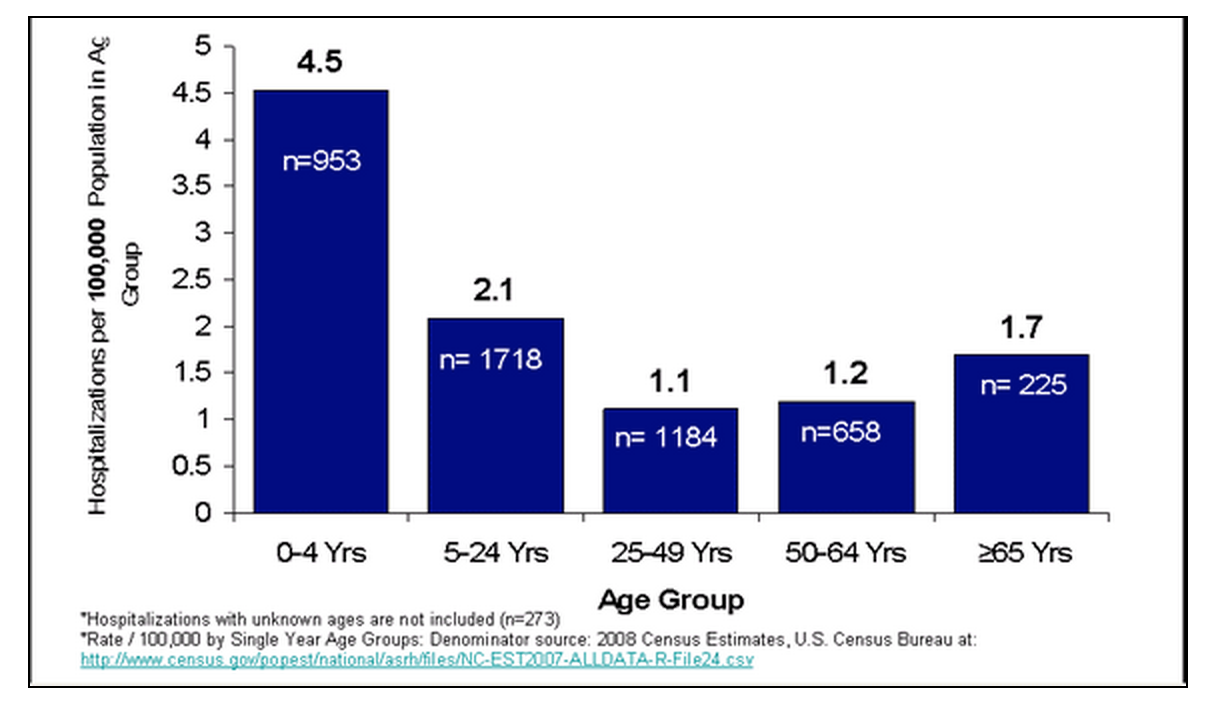
\includegraphics[width=.5\textwidth]{figures/death_graph.png}
        \caption{Mortality rates by age group \cite{deathgraph}}
	\end{figure}

    Here you can see that the death rate is relatively constant from age 25-64, so we grouped these ranges together into the ``adults'' category. The $\mu$ value for each sub-population was simply these numbers scaled by the global $\mu$ found above. The fractions of the total population that each of these sub-groups occupied \cite{pop} was found to be (.0248, .6058, 3066, .0628). Finally, the single $\beta$ had to be derived from a Next Generation Matrix. This is an equivalent of the $B0$ value for multiple sub-populations with transitions between each. This is defined to be that the jth column represents the average number of infections of individuals of type i from an individual of type j \cite{SIR}. These values were largely hand-picked for the 4 sub-population model, but we tried not to deviate too far from 1.5.
    \[
        R0 =
        \begin{bmatrix}
        3.00 & 0.10 & 0.10 & 0.10 \\
        0.10 & 3.00 & 1.00 & 0.10 \\
        2.00 & 2.00 & 1.50 & 1.00 \\
        0.10 & 0.10 & 0.50 & 1.00
        \end{bmatrix}
    \]

\subsection{Predictions}
	Running the $sir_{04}.m$ script to solve the system of ODE's for the segmented SIR model with equal distribution of vaccines produces the following plots:

    \begin{figure}[H]
    \centering
        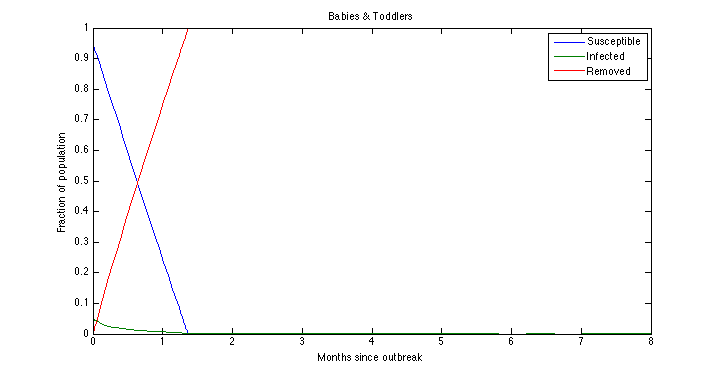
\includegraphics[width=\textwidth]{figures/ryan_plot_01.png}
    \end{figure}
    \begin{figure}[H]
    \centering
        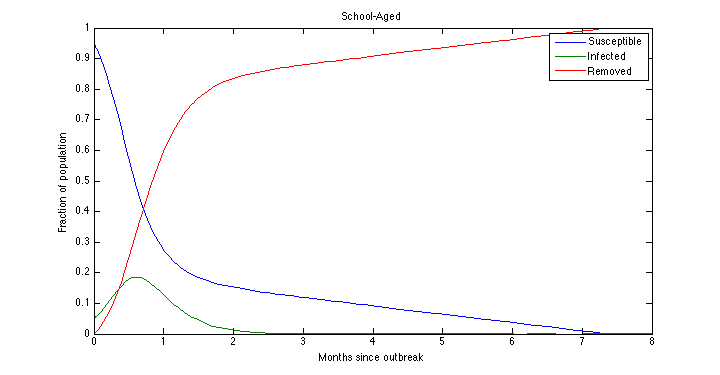
\includegraphics[width=\textwidth]{figures/ryan_plot_02.png}
    \end{figure}
    \begin{figure}[H]
    \centering
        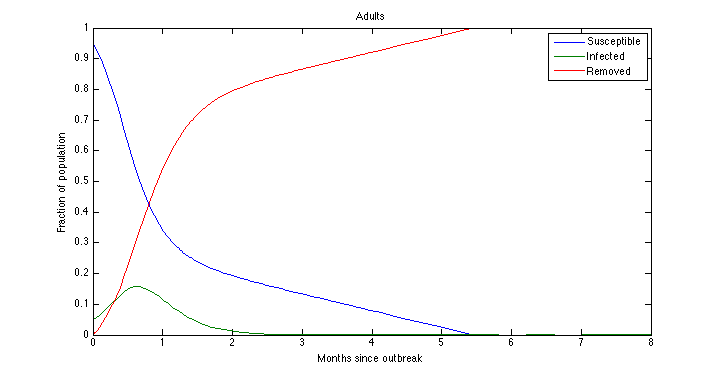
\includegraphics[width=\textwidth]{figures/ryan_plot_03.png}
    \end{figure}
    \begin{figure}[H]
    \centering
        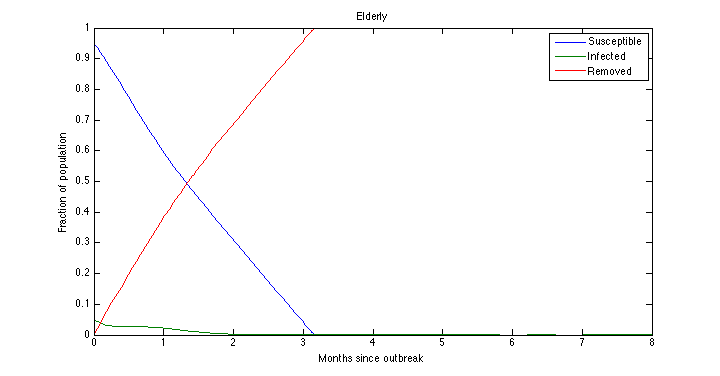
\includegraphics[width=\textwidth]{figures/ryan_plot_04.png}
    \end{figure}

    The fraction of deaths remains small for all populations so it is not plotted. The total number of person-months of suffering is the integral of the green curve.

    Running this with vaccine distributions (.1, .4, .4, .1) results in the following MATLAB output:

    \begin{lstlisting}
        total_deaths =

            0.0030    0.2532    0.0529    0.0049


        total_suffering =

            1.0e+03 *

            0.0389    7.0540    3.0925    0.1686
    \end{lstlisting}

    Running this with vaccine distributions (.4, .1, .1, .4) results in the following MATLAB output:

    \begin{lstlisting}
        total_deaths =

            0.0020    0.2674    0.0579    0.0039


        total_suffering =

            1.0e+03 *

            0.0263    7.4504    3.3864    0.1356
    \end{lstlisting}
    Running this with vaccine distributions (.1, .4, .4, .1) and $\mu = \mu * 20$results in the following MATLAB output:

     \begin{lstlisting}
        total_deaths =

            0.0598    5.0633    1.0570    0.0979


        total_suffering =

            1.0e+03 *

            0.0389    7.0522    3.0919    0.1685
    \end{lstlisting}

    Running this with vaccine distributions (.4, .1, .1, .4) and $\mu = \mu * 20$results in the following MATLAB output:

    \begin{lstlisting}
        total_deaths =

            0.0403    5.3464    1.1572    0.0787


        total_suffering =

            1.0e+03 *

            0.0263    7.4485    3.3857    0.1356
    \end{lstlisting}
% \subsection{Analysis of Model (robustness)}
% 	//TODO
% \subsection{Strengths and Weaknesses}
% 	//TODO
% \subsection{Future Work}
% 	//TODO

\section{Deterministically Allocating Vaccines Between Disjoint Populations}

First, we propose a deterministic model which doesn't divide the population
	into sections at all.
This model will help give us an idea of what the effect of dividing
	the population into sections will be.
In addition, it can give us an idea of how vaccination affects the spread of
	disease within a population.

\subsection{Disease Spread with No Vaccine}

We include this derivation of the logistic model for disease spread
	to compare with our derivation of the modified logistic model
	for disease spread and vaccination.

Suppose there are two groups of people, with $I$ representing the number of
	infected people, and $S$ represnting the number of people seceptible for the
	disease.
Suppose the probability of a single healthy person becoming sick is proportional
	only to the total number of sick people.
Since there are $S$ healthy people, the expected number of healthy people
	who become sick should be proportional to $S I$.
This model does not take into account recovery from sickness.
If we introduce a parameter $r$, we can express this relationship as a system
	of differential equations:

\begin{align*}
\frac{dS}{dt} & = - r S I \\
\frac{dI}{dt} & = r S I \\
\end{align*}

Notice that the total number of people, $S + I$, is conserved, i.e.,

\[ \frac{d}{dt} \left( S + I \right) = \frac{dS}{dt} + \frac{dI}{dt}
	= r S I - r S I = 0 \]

If we introduce another parameter, $K$, to represent the total population,
	such that $S + I = K$ for all time, then the differential equations
	can be decoupled:

\begin{align*}
\frac{dS}{dt} & = - r S (K - S) \\
\frac{dI}{dt} & = r (K - I) I \\
\end{align*}

The two differential equations shown here are now two independant, uncoupled
	differential equations which we can solve seperately.

\subsubsection{Nondimensionalizing the Model}

It would be helpful to make all of the constants dimensionless parameters.
This will give us insight into the different scales that the model works at.

To turn $I$ into a dimensionless parameter, we can divide by $K$.

\begin{align*}
\frac{d\left(\frac{I}{K}\right)}{dt}
	& = \left( r K \right) \left( \frac{I}{K} \right) \left( 1 - \frac{I}{K} \right)\\
\frac{d\widetilde{I}}{dt}
	& = \widetilde{r} \widetilde{I} \left( 1 - \widetilde{I} \right)
\end{align*}

This shows that the dynamics of $I$ do not depend on its size.
For each value of the dimensionless constant $\widetilde{r}$,
	we determine the behavior from it.

\subsection{Diease Spread with Vaccine}

Suppose we introduce a third group, $V$ for vaccinate, representing people who are
	immune from the diesease.
Right now, the only way to become immune is through vaccination,
	but we may add recovery in subsequent models.
Suppose we randomly vaccinate members of the healthy population,
	a constant number each time step.
This introduces a third parameter, $r_v$, the rate of vaccinations.
The vaccinated population isn't seceptible to the disease.
This process is modeled by the following system of diffential equations:

\begin{align*}
\frac{dI}{dt} & = r S I \\
\frac{dS}{dt} & = - r S I - r_v \\
\frac{dV}{dt} & = r_v
\end{align*}

This model is accurate only if all three of the populations remain
	positive.
This is important to remember.
The number of healthy people will always be decreasing, so once
	the number of healthy people hits zero, we stop the model.
The sick people stay sick, and the vaccinated people stay vaccinated.

The number of vaccinated people as a function of time is:

\[ V(t) = r_v t \]

Again, we find the conserved quantity $\left( S + I + V \right)$ and
	name it $K$.
For the model to be valid, we need $S = K - I - V \geq 0$.
Therefore, the model is valid as long as:

\[ K \geq I + r_v t \]

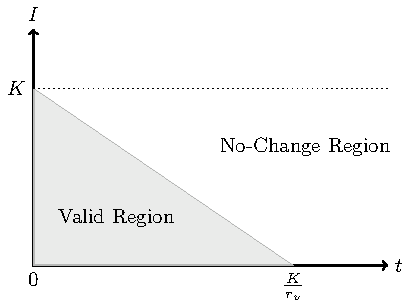
\includegraphics[width=0.5\textwidth]{figures/admissible-region.pdf}

In the above figure, once $I(t)$ hits the diagonal line,
	it stays horizontal and keeps its value.

We have now made these differential equations independant,
	within the model's zone of validity:

\begin{align*}
\frac{dI}{dt} & = r I \left( K - I - r_v t \right)\\
\frac{dS}{dt} & = - r S \left( K - S - r_v t \right) - r_v \\
\frac{dV}{dt} & = r_v t
\end{align*}

We present a solution for $I(t)$ \cite{walph}:

\begin{align}
I(t) & =
	\frac{e^{ r t (K - \frac{ r_v t}{2})}}
	{\frac{1}{S(0)} + \sqrt{\frac{\pi r}{2 r_v}}
		e^{\frac12 \left( \frac{r}{r_v} \right) K^2}
		\left(\erf\left(  \sqrt{\frac{r}{2 r_v}} (r_v t - K ) \right)
			- \erf\left( - \sqrt{\frac{r}{2 r_v}} K \right) \right)}
\end{align}

From the above expression for the boundary of the valid region,
	we get the following implicit expression for $t_f, I(t_f)$

\begin{align}
I(t_f) =
	\frac{e^{ r t_f (K - \frac{ r_v t_f }{2})}}
	{\frac{1}{S(0)} + \sqrt{\frac{\pi r}{2 r_v}}
		e^{\frac12 \left( \frac{r}{r_v} \right) K^2}
		\left(\erf\left(  \sqrt{\frac{r}{2 r_v}} (r_v t_f - K ) \right)
			- \erf\left( - \sqrt{\frac{r}{2 r_v}} K \right) \right)}
	& = K - r_v t_f
\end{align}

Here is a family of values of $I(t)$.
The total population and the rate of distributing vaccines are
	held constant, while each curve corresponds to a different
	value of the growth rate constant.
Each curve starts with an initial condition at 5 percent of the
	population, and the growth rate determines how many people
	overall are infected.

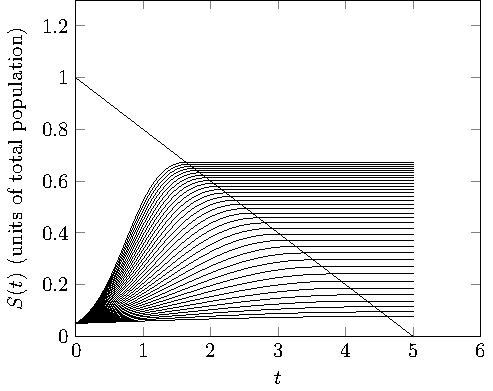
\includegraphics[width=0.5\textwidth]{figures/vaccination-model-curves-varying-s.pdf}


\subsection{Pareto Optimizing Between Two Independent Populations}

The model above modeled how one population responds to a combination
	of disease spreading and vaccines.
The model depends on $K$, the total population, $I(0)$, the initial
	number of sick people, $r$, the rate of infection growth,
	and $r_v$, the vaccination rate.
Of these parameters, in a real world setting, we can expect to know $K$
	very precicely from census data, approximate $I(0)$ as small,
	have very little idea about $r$, and control $r_v$.

I want to extend this problem to two independant populations.
Each population will get different sets of constants,
	$K_1$ and $K_2$, $I_1(0)$ and $I_2(0)$, $r_1$ and $r_2$.
The goal will be to figure out how to optimally allocate the
	vaccines between the two populations.
The decision variable, $d$, will be the fraction of the total vaccination
	rate I allocate to each population.
Population 1 will be vaccinated at a rate $d r_v$, while population
	2 will be vaccinated at a rate $(1 - d) r_v$.
In this model, I try to minimize the final number of sick people in
	each population.
This will give me a pareto front.

The following collection of pareto fronts comes from keeping the disease
	growth rate the same for both, and varying its magnitude.

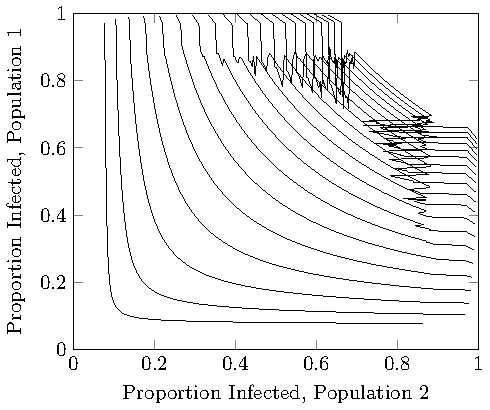
\includegraphics[width=0.5\textwidth]{figures/vaccination-model-same-r-pareto-curves.pdf}

This collection of pareto fronts comes from keeping the growth
	rate for population 2 the same, and varying the growth
	rate of population 1.

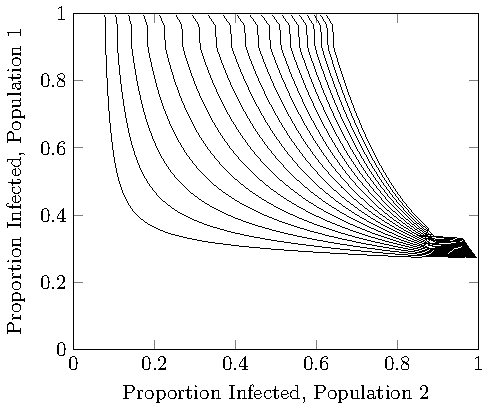
\includegraphics[width=0.5\textwidth]{figures/vaccination-model-different-r-pareto-curves.pdf}

\subsection{Improved Model}

In the preceding model, once people became infected, they stayed
	infected for the duration of the run.
The following model adds a parameter, the ``curing rate'' $\gamma$,
	which represents the rate at which individuals in the sick population
	recover (and join the removed population).
This will be the inverse of the time spent sick, which is on average
	1 week \cite{CIC-stats}.
The value of the interaction parameter $\beta$ is determined in \textbf{PLACEHOLDER}
This model is the SIR model, and has standard parameters:

\begin{align*}
\frac{dI}{dt} & = \frac{ \beta S I}{N} - \gamma I\\
\frac{dS}{dt} & = -\frac{\beta S I}{N} - r_v \\
\frac{dR}{dt} & = r_v + \gamma I
\end{align*}

We can use this model for pareto optimization.
Cornell's population is about 21,000 \cite{cornellpop},
	while ithaca's population is about 30,000 \cite{census}.
Given a rate of vaccine distribution, by integrating the equations
	we can determine how many total infections there are.
If we had 4000 vaccinations to distribute, we can make a pareto
	curve by plotting the set of points corresponding to different
	relative distributions of the vaccinations.

If one of the populations vaccinates all of its seceptible individuals
	before the other, we need to decide what to do with the vaccines
	that it is not consuming.
If we choose not to redistribute them, the pareto curve looks like this:

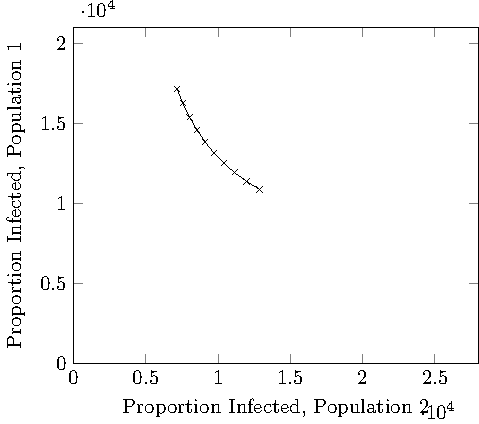
\includegraphics[width=0.5\textwidth]{figures/sir-pareto.pdf}

If we choose to redistribute them, for $\beta = 6$ and $\gamma = 4$,
	the curve looks like this:

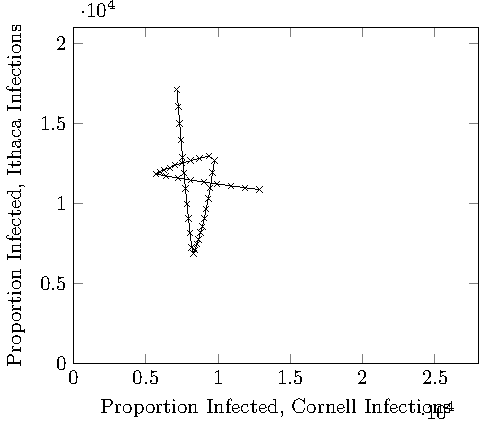
\includegraphics[width=0.5\textwidth]{figures/sir-pareto-top.pdf}

And the pareto curve looks like:

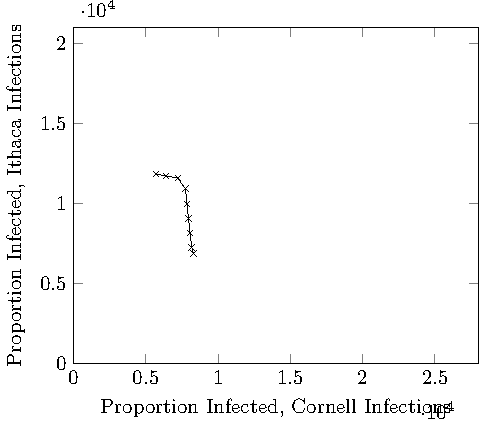
\includegraphics[width=0.5\textwidth]{figures/sir-pareto-top-pareto.pdf}

We conclude that making sure that all of the vaccines are allocated is very
	important for any vaccine model, noting the difference.
The pareto-optimal points are when 71-84\% of the vaccine goes to the
	cornellians and 29-16\% goes to the ithacans,
	and when 15-20\% of the vaccine goes to the cornellians
	and 80-85\% of the vaccine goes to the ithacans.

\subsection{Coupling the Populations}

Consider the following modifications to the model, to add interactions.
Let $\alpha$ be the interaction coefficient.
$\alpha$ should be approximately a fraction of $\beta$.
For example, if a member of one population is one tenth as likely
	to interact with the other as with one from their own population,
	the value for $\alpha$ would be $\frac{\beta}{10}$.
It represents how likely the seceptible of $i$ are to be infected by the
	infected of $j$.

\begin{align*}
\frac{dI_1}{dt} & = \frac{ \beta S_1 I_1}{N_1} + \frac{ \alpha S_1 I_2 }{N_2} - \gamma I_1\\
\frac{dS_1}{dt} & = -\frac{\beta S_1 I_1}{N_1}  - \frac{ \alpha S_1 I_2 }{N_2} - r_v \\
\frac{dR_1}{dt} & = r_v + \gamma I_1 \\
\frac{dI_2}{dt} & = \frac{ \beta S_2 I_2}{N}  + \frac{ \alpha S_2 I_1 }{N_1} - \gamma I_2\\
\frac{dS_2}{dt} & = -\frac{\beta S_2 I_2}{N}  - \frac{ \alpha S_2 I_1 }{N_1} - r_v \\
\frac{dR_2}{dt} & = r_v + \gamma I_2
\end{align*}

This model, in the fully interacting case, produces the following pareto curve:

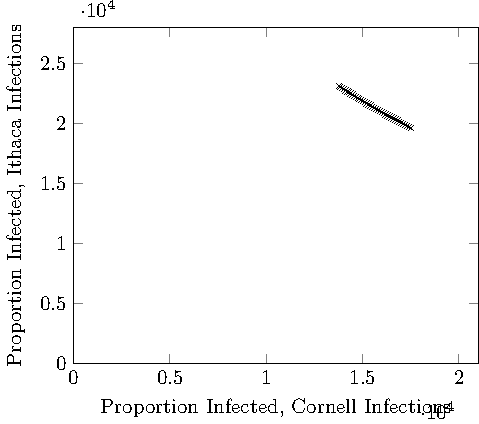
\includegraphics[width=0.5\textwidth]{figures/sir-interacting.pdf}

This doesn't show a significant variance across different immunization strategies.
It seems like vaccinating one population, and then the other, is a reasonable
	immunization strategy.
If we want to be in the middle, that is alright.


\section{Stochastic Model}
\subsection{A naive model}
\par At first, we made a simple, arbitrary stochastic model just to get a rough idea of how the disease would spread. Over the course of 5 months, we would look at the spread of the disease given certain conditions. Every citizen fell into an age category, according to demographic figures from \emph{areaConnect} \cite{areconnect}. Then, to model the spread, we associated arbitrary recovery rates, complication rates and number of people talked to per month to each age group, giving us the following table:
\begin{figure}[h!]
\centering
\begin{tabular}{c|c|c|c|c}
Age group & Heal rate & Complication chance & Connectivity & Population percentage\\ \hline
Kids & 0.5 & 0.2 & 20 & 10\%\\
Teens & 0.4 & 0.1 & 30 & 40\%\\
Adults & 0.3 & 0.3 & 25 & 40\%\\
Seniors & 0.2 & 0.7 & 10 & 10\%
\end{tabular}
\caption{Initial citizen attributes}
\end{figure}

\par The Heal rate and Complication chance columns represent the odds of a given citizen to recover from the disease in a month. The Connectivity column represents the number of people each sick citizen has a chance to infect, uniformly sampled from the entire population. We would then infect 500 people initially, and let the simulation run its course. In this particular example, we vaccinate randomly. We also assume that a person who has been sick cannot be sick again, and that when complications arise in a given patient, they are taken to the hospital and do not keep infecting the rest of the population. Here's how the spread of disease looks:
\begin{figure}[h!]
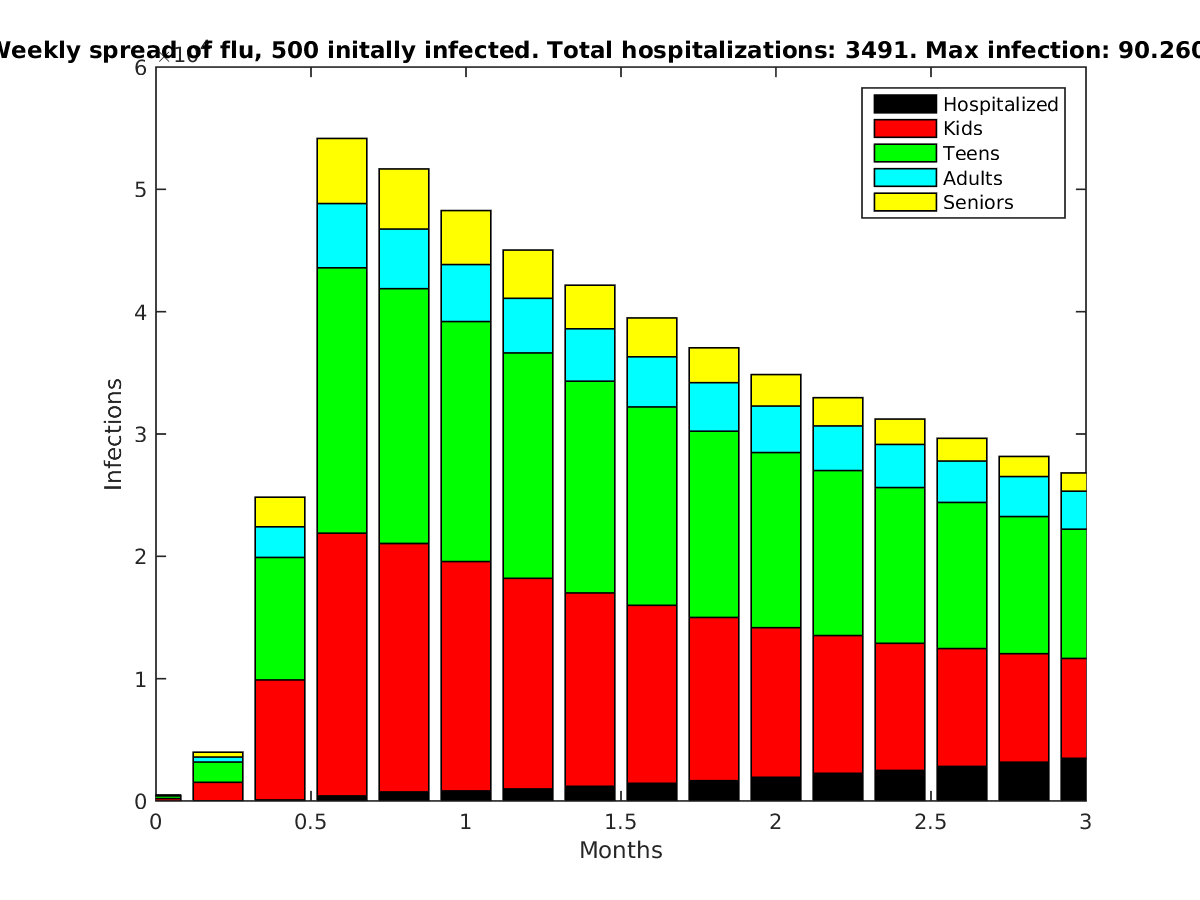
\includegraphics[width=\textwidth]{figures/Naive-model.png}
\caption{Initial model predictions}
\end{figure}
The parts of each bars represent the respective number of citizens in a given age group that are sick. The black bars on the bottom represent how many people have been hospitalized so far.
\par Unfortunately, research and according to sources from the CIC \cite{CIC-stats} \cite{CIC-qa} exposed many flaws in this model. Mostly the fact that the odds of a given citizen staying sick for more than a month are extremely low, unlike in this model where they are actually quite high. In fact, every age range stays sick for just about the same amount of time, with seniors sick for 2 weeks. The CIC data also exposed something very interesting, which is that seniors are not the ones in the most danger from the flu, kids smaller than the age of 5 are. This gave us reason to use a model that looks at the spread of the disease on a weekly basis.

\subsection{A more justified approach}
\par As mentioned in earlier, the CIC data gave us a lot to think about in terms of refining this model. First of all, we looked at the effects of the population of children in Ithaca, where children are citizens younger than 5 years of age. Since their risks of complications are so much higher, a good idea would be to immediately vaccinate all of them to avoid a devastating death toll. Fortunately, according to \emph{areaConnect}, there are less than 2,000 children in Ithaca, meaning that they can all be vaccinated as soon as the shipment of vaccines arrives. This also means that we can cut out an entire segment of the population, and generalize citizens younger than 25 years of age to a single slice. As a slight additional adaptation, we also make it such that any given citizen is more likely to talk to people from their age slice.
\par Secondly, we obtained more concrete data on how long citizens stay sick, and the likelihood of complications. The data we found was given in terms of weeks, so we changed the model to compute the spread on a weekly basis. For averaging and rounding, we assumed that there are 4 weeks in a month, and that all citizens, regardless of age, have a 90\% of healing every week. According to the CIC, a patient infected by the H1N1 virus is only contagious when showing symptoms. Therefore a citizen only infects other citizens when they are sick. Given what we know about the H1N1 virus and how contagious it is, we take 80\% to be the chance that a sick citizen infects a healthy one, with the 20\% accounting for sanitary precautions like hand sanitizer (assuming people don't have ``Swine flu Parties'' \cite{CIC-qa}).
\par With this in mind, we adapted the model such that each age group had the attributes listed in Figure~\ref{fig:justified-values}:

\begin{figure}[h!]
	\centering
	\begin{tabular}{c|c|c|c|c}
		Age group & Heal rate & Complication chance & Connectivity & Population percentage\\ \hline
		Junior & 0.9 & 0.05 & 25 & 60\%\\
		Adults & 0.9 & 0.2 & 15 & 30\%\\
		Seniors & 0.9 & 0.75 & 5 & 10\%
	\end{tabular}
	\caption{More justified attributes for age groups}
	\label{fig:justified-values}
\end{figure}

Here are a handful of runs for different vaccination strategies:
\begin{figure}[h!]
	\centering
	\begin{subfigure}[b]{0.5\textwidth}
		\centering
		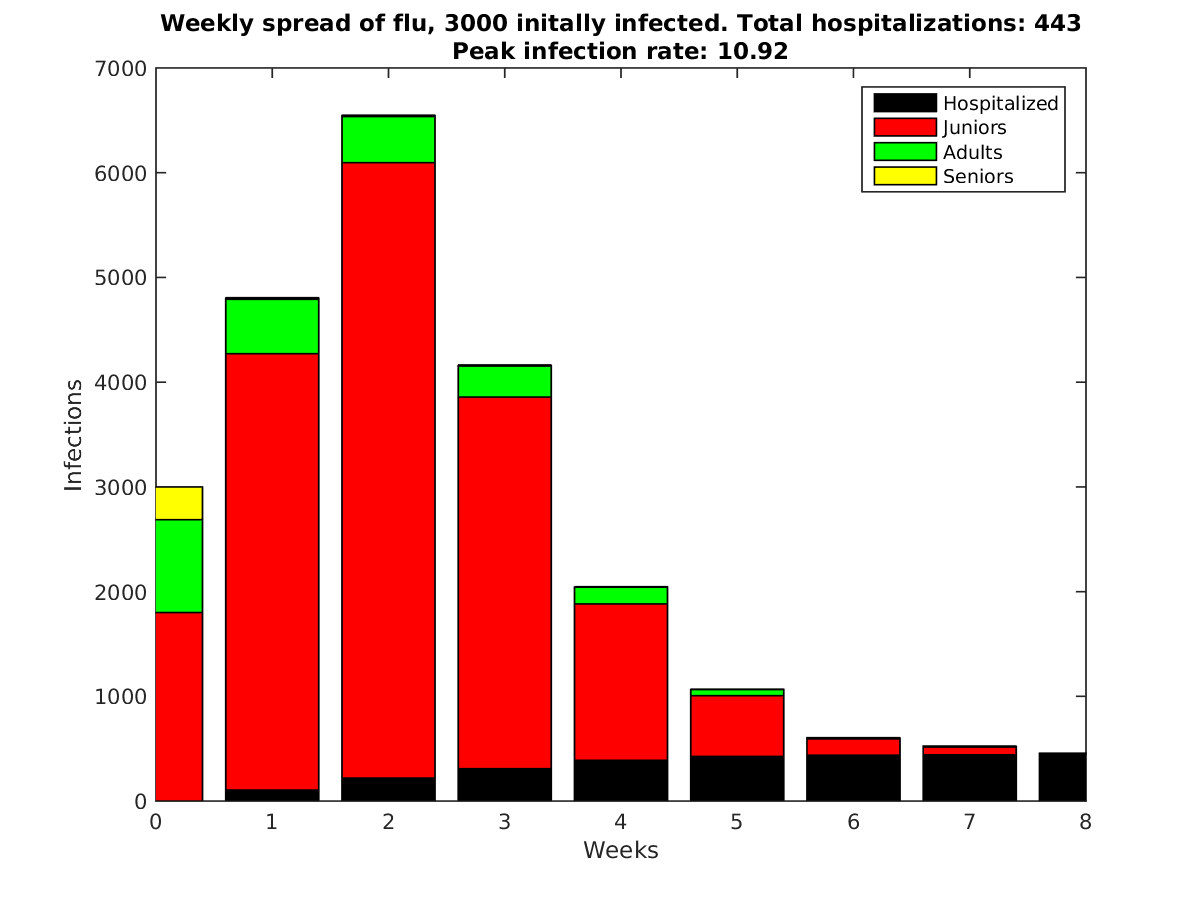
\includegraphics[width=\textwidth]{figures/Weekly-novax.png}
		\caption{No vaccination policy}
	\end{subfigure}~
	\begin{subfigure}[b]{0.5\textwidth}
		\centering
		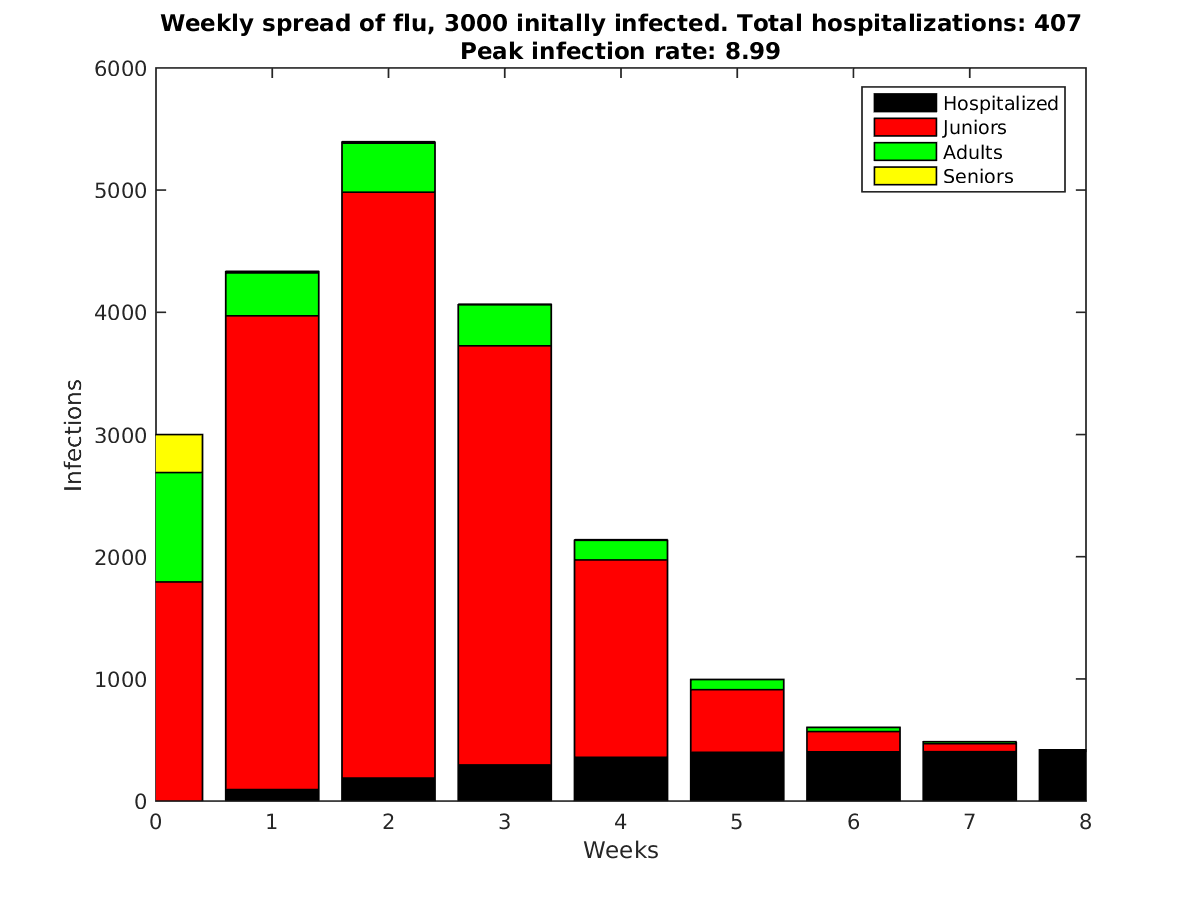
\includegraphics[width=\textwidth]{figures/Weekly-randvax.png}
		\caption{Random vaccination policy}
	\end{subfigure}\\
	\begin{subfigure}[b]{0.5\textwidth}
		\centering
		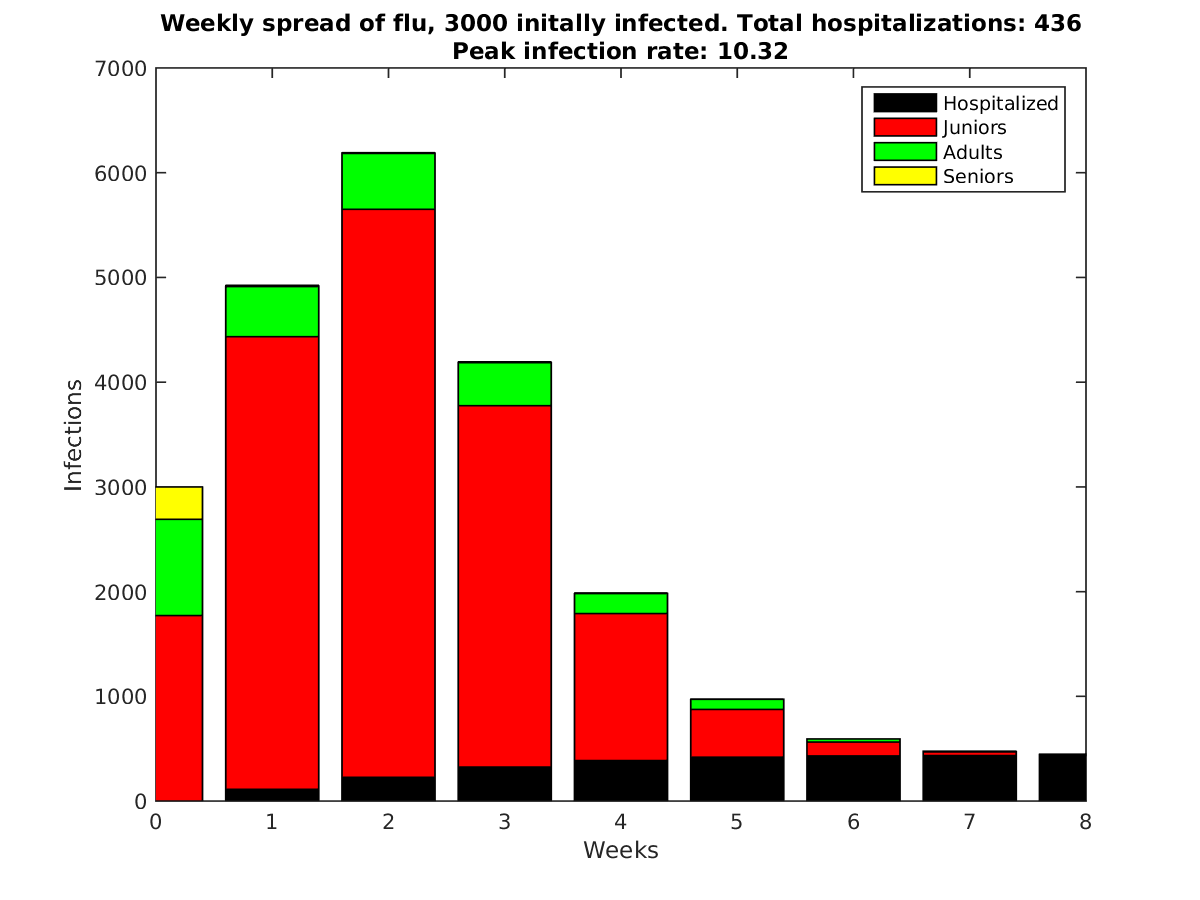
\includegraphics[width=\textwidth]{figures/Weekly-juniors.png}
		\caption{Prioritization of kids and teens}
	\end{subfigure}~
	\begin{subfigure}[b]{0.5\textwidth}
		\centering
		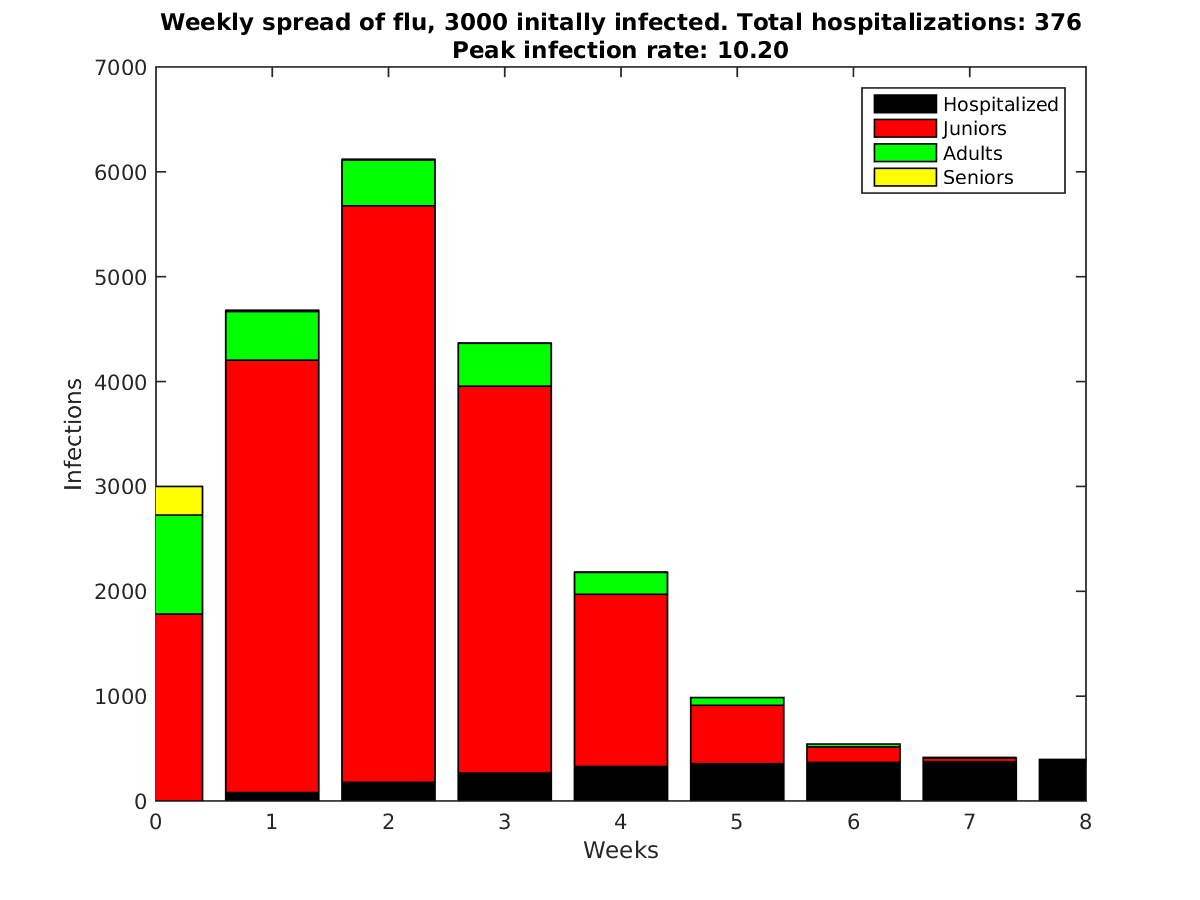
\includegraphics[width=\textwidth]{figures/Weekly-seniors.png}
		\caption{Prioritization of seniors}
	\end{subfigure}
	\caption{Model runs}
	\label{fig:modelout}
\end{figure}

Which unfortunately doesn't look promising. When the disease is twenty times as deadly, hospitalization rates scale up accordingly, and vaccination policies keep their effectiveness.

\subsection{Analysis}
\par As we saw in Figure~\ref{fig:modelout}, vaccination policies don't actually impact the spread of the disease too much. Rather, it seems to be more helpful for damage control. We see from the 4 graphs in Figure~\ref{fig:modelout} the peak infection rate seems to stay near 10\% regardless of the vaccination policy. On the other hand, it seems to help for damage control because even though the infection rate stays the same, when we vaccinate more seniors, fewer people end up hospitalized than when we target more juniors. But surprisingly, the random vaccination policy consistently came out on top. This peaked our interest, so we ran many simulations comparing the three models. Figure~\ref{fig:10outs} shows the outputs side by side. We see that the random policy actually puts just about as many people in the hospital as the policy that targets seniors, while keeping the peak infection rate actually lower than all the policies. When the disease is deadlier, all models agree that the random policy is better than all.
\par Consensus on how long a given epidemic should last is about 2 months, and it seems that our model agrees, so we can at least verify that it decently approximates a real spread.
\par Part of the reason why the different methods don't have such a different outcome seems to be that the disease simply spreads too fast. Long before enough vaccinations can be handed out, the infection has spread too far for it to be slowed down.

\begin{figure}[h!]
\centering
\begin{subfigure}[b]{0.5\textwidth}
\centering
\begin{tabular}{rc|c}
& Peak infection (\%) & Total hospitalizations\\ \cline{2-3}
& 11.1  & 431\\
& 10.62 & 418\\
& 9.47  & 433\\
& 8.9   & 414\\
& 11.11 & 404\\
& 10.24 & 411\\
& 11.35 & 442\\
& 10.59 & 412\\
& 10.88 & 432\\
& 10    & 395\\ \hline
Mean & 10.426 & 419.2
\end{tabular}
\caption{Juniors first}
\end{subfigure}~
\begin{subfigure}[b]{0.5\textwidth}
\centering
\begin{tabular}{rc|c}
& Peak infection (\%) & Total hospitalizations\\ \cline{2-3}
& 10.45 & 389\\
& 10.65 & 376\\
& 10.25 & 419\\
& 10.86 & 388\\
& 10.1  & 384\\
& 11.05 & 373\\
& 9.97  & 377\\
& 9.57  & 383\\
& 10.14 & 363\\
& 9.91  & 367\\ \hline
Mean & 10.295 & 381.9
\end{tabular}
\caption{Seniors first}
\end{subfigure}\\
\begin{subfigure}[b]{0.5\textwidth}
\centering
\begin{tabular}{rc|c}
& Peak infection (\%) & Total hospitalizations\\ \cline{2-3}
& 9.5   & 378\\
& 9.99  & 393\\
& 10.02 & 373\\
& 9.28  & 370\\
& 9.72  & 386\\
& 9.68  & 369\\
& 10.25 & 423\\
& 10.36 & 415\\
& 9.11  & 370\\
& 9.96  & 352\\ \hline
Mean & 9.787 & 382.9
\end{tabular}
\caption{Indiscriminate vaccinations}
\end{subfigure}
\caption{Comparison of 10 runs for different vaccination policies}
\label{fig:10outs}
\end{figure}

\section{Conclusion}
	//TODO
\section{References}
	\begin{thebibliography}{9}
	\bibitem{areconnect}
		\url{http://ithaca.areaconnect.com/statistics.htm}
	\bibitem{CIC-stats}
		\url{http://www.cdc.gov/h1n1flu/surveillanceqa.htm}
	\bibitem{CIC-qa}
		\url{http://www.cdc.gov/h1n1flu/qa.htm}
	\bibitem{walph}
		Wolfram Research Inc.,
		\emph{WolframAlpha},
		Retrieved September 26, 2015
		\url{http://www.wolframalpha.com/input/?i=ds%2Fdt+%3D+r+s+%28K+-+s+-+a+t%29}
		\url{http://www.wolframalpha.com/input/?i=%E2%88%AB+e^%28-a+x^2+%2B+b+x%29+dx}
	\bibitem{SIR}
		\url{http://web.stanford.edu/~jhj1/teachingdocs/Jones-on-R0.pdf}
	\bibitem{applet}
		\url{http://www.public.asu.edu/~hnesse/classes/sirv.html?}
	\bibitem{NGM}
		\url{http://rsif.royalsocietypublishing.org/content/7/47/873}
	\bibitem{oneweek}
		\url{https://www.cdph.ca.gov/HealthInfo/h1n1flufaqs/Pages/H1N1fluFAQs-01-GenInfo.aspx}
	\bibitem{R0}
		\url{http://www.ncbi.nlm.nih.gov/pmc/articles/PMC2715422/}
	\bibitem{deathgraph}
		\url{http://www.cdc.gov/h1n1flu/surveillanceqa.htm}
    \bibitem{init}
        \url{http://academic.udayton.edu/muhammadusman/2010Stander/H1N1.pdf}
    \bibitem{deathpercent}
        \url{http://www.cdc.gov/h1n1flu/estimates_2009_h1n1.htm}
    \bibitem{pop}
        \url{http://ithaca.areaconnect.com/statistics.htm}
	\end{thebibliography}

\section{Source Code}
	\lstinputlisting{models/stochastic/spread.m}
	\lstinputlisting{models/stochastic/random_vaccine.m}
	\lstinputlisting{models/deterministic/numerical_sir/sir_04.m}
	\lstinputlisting{models/deterministic/numerical_sir/sir_update_04.m}
	\lstinputlisting{models/deterministic/sir-two-coupled.m}
	\lstinputlisting{models/deterministic/logistic-newton-s-investigation.m}
	\lstinputlisting{models/deterministic/logistic-newton-s-investigation.m}

\section{Individual Contributions}
	Paul handled mostly what covered the Stochastic Model, while Chris and Ryan worked on their own deterministic models. Everyone did a lot of their work in the presence of everyone else, while still putting in a lot of time at home. When it came time to submit, everyone was ready to work. All in all, lots of work put in from all team member and we were all satisfied with each other's work.

\end{document}